\renewcommand{\chaptername}{Redes}  
\graphicspath{{parte_2/redes/}}
\chapter{Redes}
\markright{\chaptername }

% resumen del capitulo 
\begin{center}
	\begin{tcolorbox}[colback=gray!5!white, %Color del fondo
		colframe=blue!75!black,
		title= \center{\Large{resumen}} ]
		Se definen los componentes básicos de una red: los modelos OSI y TCP/IP. Luego analizamos los protocolos TCP, y DHCP,y el protocolo IP. Luego, se propone el software WireShark para ver estos protocolos funcionando sobre una red ya implementada. 

	\end{tcolorbox}
\end{center}    
\section{Introducción} 
En este capítulo analizamos las redes de computadoras,y como se conectan entre sí los dispositivos de una red. Ademas, se analizan dos modelos de capas principales: OSI y TCP/IP, donde cada uno consta de varias capas, donde se brinda un breve resumen de cada capa. 
Luego, se analizan, dos protocolos para reconocer dispositivos en una red, el protocolo DHCP,que le asigna una dirección, y el protocolo IP,que le asigna una red. Además, se introduce el concepto de sniffer, y se muestra como visualizar el contenido de los datos que están circulando en una red. Los conceptos en que profundiza el presente capítulo, son aquellos de mayor interés para la construcción del dispositivo.  


\section{Redes de Área local }
Existen tres tipos de redes: Redes de área local, de área metropolitana, y redes de área amplia. El dispositivo desarrollado en el presente trabajo, se conecta a la red de área local de la institución, por ende, es importante entender de una manera elemental el funcionamiento de las redes, sus protocolos, y sus modelos de capas.   

Las redes de área local, son aquellas que se interconectan distintos equipos de una institución, departamento de una empresa, etc, para que se realice un intercambio de información, a través de un medio. Las redes de área local, generalmente se dice que son redes LAN, por sus siglas en inglés(Local Area Network).  En general, son redes de propiedad privada. Existe un estándar, para estas redes LAN cuando se conectan de forma inalámbrica: IEEE 802.11 (comúnmente denominado WiFi), y cuando son alámbricas existe el estandar IEEE 802.7(comúnmente denominado ethernet). Las redes WiFi, no se utilizan en este trabajo, por utilizar técnicas de radiofrecuencia, que interfieren con los receptores de comunicaciones.  
En el caso de redes alámbricas, las computadoras, realizan un enlace punto a punto, a través de un dispositivo denominado \textbf{Switch}.Un switch, posee varias entradas para conectar mas de una PC,y el trabajo de este, es transmitir mensajes entre computadoras, conociendo la dirección de destino, que viene incluida en el mensaje. Si se requieren redes mas grandes, pueden interconectarse Switchs entre sí, y armar redes de mayor tamaño. 


En el presente trabajo, se conecta el dispositivo a un switch, que esta ubicado en sala de control,del Instituto Argentino De Radioastronomía. Ademas al finalizar el trabajo, se solicitará que se le asigne una dirección fija dentro de la red institucional.  

En el trabajo realizado en este presente informe, usamos un modelo conocido como arquitectura "cliente-servidor". Esta arquitectura, se basa en que hay maquinas clientes, que solicitan un servicio, a otra estación de trabajo, denominada servidor. Los clientes, son las estaciones de trabajo del lugar, y el servidor es el dispositivo desarrollado en esta tesis, ya que es el qué brinda el servicio de apuntamiento de antena. En otras palabras, las estaciones de trabajo deben conectarse al dispositivo desarrollado en el presente documento. De ahí, que se requiera el permiso correspondiente para fijar la dirección del dispositivo.  




\section{Modelo de capas}

para reducir la complejidad de las redes, se organizan en capas, donde cada capa, ofrece ciertos servicios a capas superiores, mientras les oculta detalles relacionados con la forma en que se implementan estos servicios. El uso de capas, no es un problema inherente de las redes, sino que se aplica en otros ámbitos de las ciencias de la computación. La cantidad de capas es variable, y depende del problema en cuestión. En términos de redes de computadoras, se usan dos modelos principalmente, el modelo OSI y el modelo TCP/IP. El primero consta de siete capas, el segundo consta de cinco capas. 

para entender este sistema de capas, consideramos una capa y le ponemos un numero K. Supongamos que la capa K de una PC desea comunicarse con la capa K de otra. La forma en que ambas se comunican, se denomina protocolo, que define las reglas y convenciones usadas en esta comunicación. 

\begin{wrapfigure}[21]{l}{0.4\textwidth}
	\centering 
%	\caption{Conexion entre capas.En esta figura se observan la interface,protocolo y conexionado}
	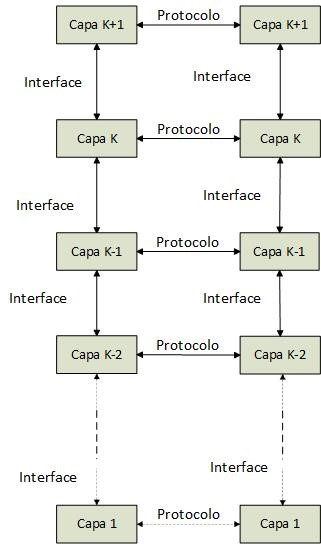
\includegraphics[scale=0.6]{modcap}
	\caption{Conexión entre capas.En esta figura se observan las interfaces,protocolo y conexionado}
	\label{fig:modOSI}	
\end{wrapfigure}
En realidad, las capas, no se comunican directamente entre sí, sino que pasan la información (datos y control) a la capa inferior (en nuestro ejemplo, capa k-1), y así, hasta el nivel mas bajo (capa 1). En el nivel mas bajo, envía la información a otra maquina dentro de la red, y ella se encarga de pasar los datos a las capas superiores, en un proceso inverso al realizado para enviar la información. La comunicación entre capas se realiza a través de una entidad denominada interface. La figura  \ref{fig:modOSI} ilustra el proceso de capas descrito.

A un conjunto de capas y protocolos se conoce como Arquitectura de Red. La especificación de una arquitectura debe contener suficiente información como para permitir que un programador escriba el programa, o construya el hardware para cada capa, de manera que se cumpla correctamente el protocolo apropiado.

Debido a que existen muchas computadoras dentro de una organización, estos protocolos, necesitan de alguna manera identificar el destinatario del mensaje y quien lo envía, esto se denomina direccionamiento o nombramiento en las capas. para realizar esto, se definen dos modelos: El modelo OSI y el modelo TCP/IP. Se diferencian en la cantidad de capas de cada modelo, los nombres de cada capa, pero la funcionalidad sigue siendo la misma: intercambiar información entre dos dispositivos, usando un esquema de capas, las cuales permiten que el diseñador tenga mas facilidad a la hora de diseñar una red. 



\subsection{Modelo OSI}
El modelo OSI, se basa en una propuesta desarrollada por la organización internacional de normas(ISO), en un intento de estandarización para los protocolos. En si, es un modelo general, pero sus protocolos no se utilizan masivamente.La sigla OSI proviene de ''open system interconection''(sistema de interconexión abierto). Este modelo tiene siete capas, y los principios utilizados para llegar a ellas son los siguientes:
\begin{enumerate}
	\item Se debe crear una capa en donde se requiera un nivel diferente de abstracción 
	\item Cada capa debe realizar una función bien definida 
	\item La función de cada capa se debe elegir teniendo en cuenta la definición de protocolos estandarizados
	internacionalmente
	\item Es necesario elegir los límites de las capas de modo que se minimice el flujo de información a través de las interfaces 
	\item La cantidad de capas debe ser suficiente como para no tener que agrupar funciones distintas en
	la misma capa; ademas, debe ser lo bastante pequeña como para que la arquitectura no se vuelva
	inmanejable. 
\end{enumerate} 
Las capas, se muestran en la figura a continuación:% \ref{fig:mod_osi}:
\vspace{-2mm}  
\begin{figure}[ht]
	\centering
	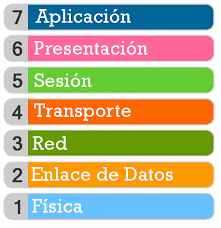
\includegraphics[scale=0.5]{modelosi} 
	\caption{Capas del Modelo OSI}
	\label{fig:mod_osi}
\end{figure}  


\subsubsection{capa 1 - Capa física} 
Esta capa, se relaciona con la transmisión de bits a través de un canal de comunicación. Los aspectos de diseño tienen que ver con las interfaces mecánica, eléctrica y de temporización, así como con el medio de transmisión físico que se encuentra bajo la capa física.


\subsubsection{capa 2 - Enlace de datos } 
La función principal es transformar un medio de transmisión puro, en una linea que esté libre de errores. Ademas, proporciona medios para activar,desactivar y mantener el enlace(es decir, la comunicación). Aquí, esta definido un componente de hardware: la tarjeta o placa de red. Cada placa de red tiene un número único conocido como MAC address, y es único para cada dispositivo en el mundo. 

\subsubsection{capa 3 - Capa de red}
La capa de red, realiza la transferencia de información entre sistemas finales, liberando a las capas superiores del conocimiento de los medios de transmisión y tecnologías de conmutación usadas. 

Si hay demasiados paquetes en la subred al mismo tiempo, se interpondrán en el camino unos con
otros y formarán cuellos de botella. El manejo de la congestión también es responsabilidad de la capa de
red, en conjunto con las capas superiores que adaptan la carga que colocan en la red.
\subsubsection{capa 4 - Transporte }
En esta capa, se reciben datos de las capas superiores, y los '' particiona'' en unidades mas pequeñas, para ser enviadas a las capa de red.Ademas,debe asegurarse  que estos paquetes lleguen a destino. En otras palabras, parte los mensajes de las capas superiores para ser transmitidas al medio de comunicación. 

\subsubsection{capa 5 - Sesión  }
Esta capa, proporciona mecanismos para el control del diálogo (decidir quien debe transmitir)entre las aplicaciones de los sistemas finales. En muchos casos, estos servicios son totalmente  imprescindibles,sin embargo, en algunas aplicaciones, su utilización es obligatoria. 

\subsubsection{capa 6 - Presentación}
Aquí, se define el formato de los datos que van a intercambiarse en las aplicaciones., y ofrece a las aplicaciones un conjunto de servicios de transformación de datos. Ejemplos específicos, son compresión y cifrado de datos. 


\subsubsection{capa 7 - Aplicación} 
Esta capa, proporciona a los programas de aplicación, un medio para que accedan al entorno OSI. Aquí, se encuentran funciones de administración, y los mecanismos para la implementación de aplicaciones distribuidas. En esta capa, tenemos las aplicaciones de uso general, como la transferencia de ficheros, correo electrónico, navegadores web,etc. 


\section{Modelo TCP/IP} 
  El modelo TCP/IP es usado para conectar computadoras entre si a través de una red interna dentro de una organización. Este modelo se muestra en la figura \ref{fig:model_tcpip}, y se dará una breve explicación de cada capa: 
  \begin{figure}[ht]
  	\centering
  	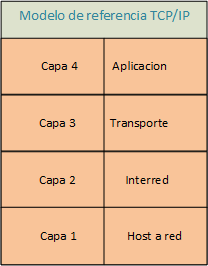
\includegraphics{model_tcpip}
  	\caption{Modelo de capas TCP/IP}
  	\label{fig:model_tcpip}
  \end{figure} 

\subsection{capa 1 - Capa de Host a red}
La capa 1,del modelo TCP/IP, también se la suele nombrar capa de enlace.En este documento utilizamos como nombre de capa ''host a red''.De esta capa, no se puede decir mucho, excepto que puntualiza que el host se debe conectar a la red mediante el mismo protocolo para que se puedan enviar paquetes IP (véase la siguiente sección). Este protocolo no está definido y varia de una red a otra.
\subsection{capa 2 - Interred}
Su trabajo es permitir que los hosts inyecten paquetes dentro de cualquier red y que viajen a su destino de manera independiente. Una analogía es el servicio de correo. Una persona, deposita una serie de cartas internacionales en un buzón, y la mayoría de ellas se entregarán en la dirección correcta del país de destino. Es probable que las cartas, viajes a través de una o mas puertas de enlace de correo internacional, pero esto es transparente a los usuarios. Este trabajo, lo realiza la capa de interred, que da transparencia a los usuarios de como viajan estos paquetes dentro de una red. 
La capa de interred, define un paquete de formato y protocolo denominado protocolo IP (Internet protocol). El trabajo de la capa de interred es entregar paquetes IP al destinatario. 

\subsection{capa 3 - Transporte}
Está diseñada para permitir que las entidades iguales en los hosts origen y destino puedan llevar a cabo una conversación. Aquí se han definido dos protocolos de transporte de extremo a extremo: el TCP (protocolo de control de transmisión), es un protocolo confiable, que permite un flujo de bytes que se origina en una máquina se entregue sin errores en cualquier otra máquina. Divide le flujo de bytes entrantes en mensajes discretos y pasa cada uno de ellos a la capa de interred. En el destino, ocurre el proceso inverso, es decir, el destino reconstruye el mensaje recibido. TCP maneja control de flujo para asegurarse que un emisor rápido no sature a un receptor lento con mas mensajes de los que puede manejar. 
El segundo protocolo de esta capa UDP (protocolo de datagrama de usuario) es un protocolo no confiable, se usa para aplicaciones que no desean la secuenciación o control de flujo de TCP y desean proporcionar el suyo. Es decir, se usa en aplicaciones donde la entrega puntual es mas importante que la precisa. 



\subsection{capa 4 - Aplicación}
Contiene todos los protocolos de nivel mas alto. Los primeros fueron TELNET, FTP, SMTP, etc. Con el tiempo, se han agregado otros protocolos, por ejemplo, HTTP, DNS, etc. 
En la siguiente imagen, se muestra la relación entre las capas del modelo TCP/IP
%\vspace{-1cm}
\begin{figure}[ht]
	\centering
	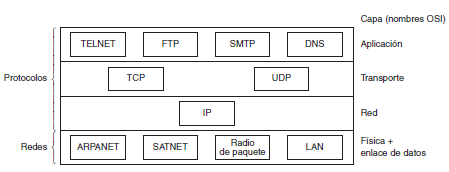
\includegraphics[height=5.0cm]{cap_ap_tcpip}
	\caption{Esquema de interconexión del modelo TCP/IP}
\end{figure}


\section{OSI vs TCP/IP }

Los dos modelos tienen mucho en común. Ambos se basan en un modelo de capas, independientes entre sí. Es importante tener en cuenta que se están comparando los modelos de referencia, no los protocolos de comunicación entre si. En la siguiente figura se muestra la comparación de las capas:  

\begin{figure}[ht]
	\centering 
	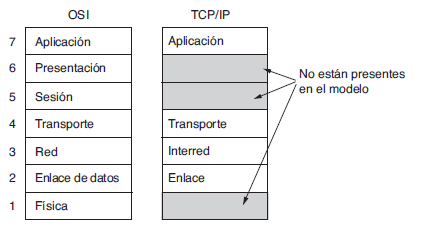
\includegraphics{comptcposi}
	\caption{Comparativa entre modelo OSI y TCP/IP}
	\label{fig:comp_tcposi}
\end{figure}

El modelo OSI, define tres partes básicas: 
\begin{enumerate}
	\item Servicios 
	\item Interfaces 
	\item Protocolos
\end{enumerate}

El modelo OSI, define bien estas tres partes, y las distingue de una manera clara, cosa que no realiza el modelo TCP/IP. Sin embargo, los protocolos del modelo OSI, son difíciles de implementar, por esto se opta por los protocolos que se definen en el modelo TCP/IP. 

Una diferencia importante, se observan en la figura \ref{fig:comp_tcposi}, en el que se observa que el modelo TCP/IP tiene cuatro capas, mientas el otro tiene siete. Una ventaja, en el modelo OSI, es que el protocolo de una capa, puede cambiarse con facilidad, sin afectar las demas capas, esto no es así en el modelo TCP/IP. 

Otra diferencia está en área de comunicación orientada a la conexión y no orientada a la conexión. El modelo OSI soporta ambas comunicaciones en la capa de transporte. Em modelo TCP/IP solo tiene un modo en la capa de red(no orientado a la conexión),pero soporta ambos modos en la capa de transporte, lo que da a los usuarios la oportunidad de elegir, en casos de protocolos sencillos de solicitud-respuesta.  




\section{Protocolo IP} 
%protocolo IP RFC 1958
La capa de red, se encarga de llevar todos los paquetes a destino. Podría ocurrir, que existan varios enrutadores en el medio. Esto contrasta con la capa de enlace de datos, que asegura la fiabilidad de un extremo a otro de un cable. El protocolo IP, se encuentra en el estandar RFC 1958, y es de acceso público. Este protocolo se denomina IP por las siglas ''Internet Protocol''. 

La comunicación en internet funciona de la siguiente manera: la capa de transporte, fragmenta los datos de la capa superior, y se los transmite a la capa de red. Los enrutadores, reenvian cada paquete, a través de mas de un enrutador, hasta llegar a destino. En el destino, la capa de red entrega los datos a la capa de transporte y se los envía a la capa de aplicación. Cuando todas las piezas llegan finalmente a la máquina de destino, la capa de red las vuelve a ensamblar para formar el datagrama original. Un datagrama es la información que viaja en una red, y esta compuesta por números binarios. Si bien, esta definición es bastante burda, es suficiente para el presente trabajo. El datagrama IP, se muestra en la figura siguiente 
% datagrama Ip 

\begin{figure}[ht]
	\centering
	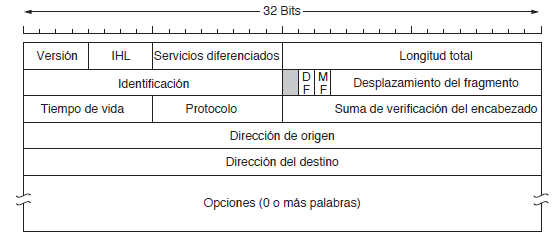
\includegraphics{parte_2/redes/datagip}
	\caption{Datagrama IP}
	\label{fig:datIP}
\end{figure} 
Este datagrama, se compone de dos partes: encabezado y carga útil. El encabezado, se compone de 20 bytes fija y una parte opcional de longitud variable. Los bits se transmiten de izquierda a derecha, y de arriba hacia abajo en la figura \ref{fig:datIP}. Todos los parámetros, están definidos en el estándar mencionado al principio de esta sección, en este trabajo, solo nos concentramos en dos parámetros: Dirección origen y Dirección destino. Estas son las que debemos utilizar para configurar el software, y que las estaciones de trabajo puedan conectarse a nuestro dispositivo. Estas direcciones, se conocen como direcciones IP. 
\subsection{Direcciones IP} 
Si se observa, la figura \ref{fig:datIP}, se observa que hay 32 bits(o 4 bytes) para indicar esta direcciones. Estas direcciones están compuestas de una porcion de longitud variable para indicar la red en los bits superiores, y de una porcion de host en los bits.La porción de red tiene el mismo valor para todos los hosts en una sola red, como una LAN Ethernet. Esto significa que una red corresponde a un bloque contiguo de espacio de direcciones IP.A este bloque se le llama prefijo. 

Las direcciones IP se escriben en notación decimal con puntos. En este formato, cada uno de los 4 bytes se escribe en decimal, de 0 a 255. Por ejemplo, la dirección hexadecimal 80D00297 de 32 bits se escribe como 128.208.2.151.  
inferiores. para escribir los prefijos, se proporciona la ip menor en el bloque y tamaño del mismo. El tamaño se determina mediante el número de bits en la porción de red, los restantes bits(bits de host) pueden variar. Esto significa, que el prefijo debe ser potencia de dos. Por convención, el préfijo se escribe despues de la ip, con los bits dedicados a los host. Por ejemplo, la siguiente notación 128.208.0.0/24, significa que hay 24 bits para la red, y 8 bits para el host. 

Como el prefijo que indica la red, puede ser de longitud variable, entonces se debe realizar una operación and binario con un numero de unos en la parte de red, y ceros restantes.Este número con el que se realiza esta operación, se denomina \textbf{mascara de subred}. En el ejemplo anterior: 128.208.0.0/24, la mascara de subred es en decimal: 255.255.255.0. Si realizamos la operación and bit a bit entre 255.255.255.0 y 128.208.0.0, obtenemos 128.208.0.0, lo cual indica que pertenece a la red 128.208.0.0. En este trabajo, solo requerimos de estos conceptos, para configurar el software de cada estación de trabajo, y realizar la conexión con el dispositivo desarrollado en el presente trabajo.     
 
\section{Protocolo DHCP} 

De la sección anterior, se obtiene que cada computadora, estación de trabajo, o dispositivo que se conecte a la red, debe al menos configurarse la dirección IP, y la mascara de subred, para que puedan intercambiar mensajes entre ellos, o utilizar cualquier servicio disponible en la red. Esto, puede resultar un proceso tedioso, por esto, se define en el estándar RFC 2131 un protocolo de asignación dinámicas de ips, conocido como DHCP(Protocolo de Configuración Dinámica de Host,
del inglés Dynamic Host Configuration Protocol). En el estandar, están definidas la forma de comunicación para obtener estos datos, que es básicamente la dirección IP asignada de manera automática.  
Dentro de cada red, debe existir un servidor DHCP. para iniciar la solicitud, la máquina, envía a través de la red, una solicitud, denominada DHCPDISCOVER.Si el servidor esta disponible, envía la dirección en un paquete denominado DHCPOFFER. 
Un paquete DHCP esta conformado por los bits que se muestran en la figura \ref{fig:pqdhcp}: 
\begin{figure}[ht]
	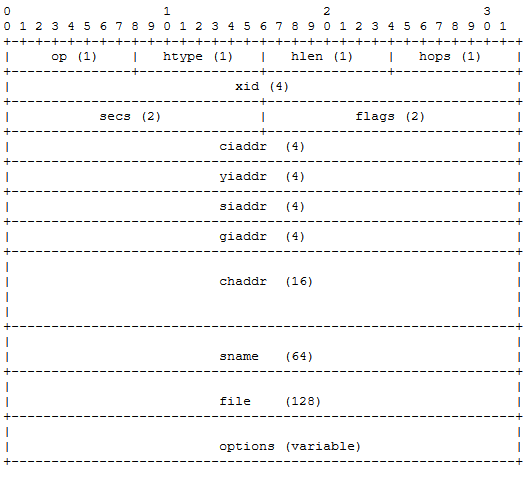
\includegraphics[width=\textwidth,height=10cm]{paqdhcp}
	\caption{Datagrama para intercambio de mensajes del protocolo DHCP}
	\label{fig:pqdhcp}
\end{figure} 

Estos parámetros, son bits, los cuales deben enviarse a través de la red. Estos campos de bits, no serán explicados, ya que están implementados dentro de la libreria W5100 que maneja el entorno de arduino UNO. Estos bits están descritos en el estándar indicado en el primer párrafo de la esta sección, y son de acceso público. 


\section{Protocolo TCP } 
Este protocolo, pertenece a la capa de transporte. Se diseño especificamente para proporcionar un flujo de bytes confiable de extremo a extremo a través de una interred no confiable. Una interred difiere de una sola red debido a que sus diversas partes podrían tener diferentes topologías, anchos de banda, retardos, tamaños de paquete y otros parámetros. TCP se diseñó para adaptarse de manera dinámica a las propiedades de la interred y sobreponerse a muchos tipos de fallas.

%para conocer la importancia de este protocolo dentro de las redes, se ha definido el primer estandar RFC 793, en el año 1981. Luego de este documento, se han definido varias mejoras: 
%\begin{enumerate}
%	\item RFC 1122: aclaraciones, y correcciones de errores  
%	\item RFC 1323: extensiones para alto desempeño 
%	\item RFC 2018: confirmaciones de recepción selectivas 
%	\item RFC 2581:control de congestión 
%	\item RFC 2873 readaptacion de los campos del encabezado para la calidad del servicio 
%	\item RFC 2988: temporizadores de transmisión mejorados 
%	\item RFC 3168: notificación explícita de congestión 
%\end{enumerate} 

%Las normas RFC, son solo algunas de las relacionadas al protocolo TCP.Debido a la gran cantidad de normas generadas para este protocolo, se ha definido un nuevo documento que los ordena a todos estos:el RFC 4614.  

La capa IP no ofrece ninguna garantía de que los datagrama se entregarán de manera apropiada, ni tampoco una indicación sobre qué tan rápido se pueden enviar los datagrama. Corresponde a TCP enviar los datagramas con la suficiente rapidez como para hacer uso de la capacidad sin provocar una congestión; también le corresponde terminar los temporizadores y retransmitir los datagramas que no se entreguen. 

\subsection{Servicio TCP}
	El servicio TCP se obtiene al hacer que tanto el servidor como el receptor creen puntos terminales, llamados sockets. Cada socket tiene un número (dirección) que consiste en la dirección IP del host y un número de 16 bits que es local para ese host, llamado puerto. Un puerto, es definido por la capa de aplicación, que es el punto de acceso a la capa de aplicación. para obtener el servicio TCP, hay que establecer de manera explícita una conexión entre un socket en una máquina y un socket en otra máquina. 
	Existen puertos que se denominan ''conocidos'', y son casi un estándar, por ejemplo el puerto 80 para el protocolo HTTP. Los puertos definidos van de 0 a 1024. Los puertos de 1024.Los puertos desde el 1024 hasta el 49151 son puertos que se pueden registrar en IANA, pero las aplicaciones son las que seleccionan sus propios puertos.  
	Todas las conexiones TCP son full dúplex y de punto a punto. Full dúplex significa que el tráfico puede 	ir en ambas direcciones al mismo tiempo. Punto a punto significa que cada conexión tiene exactamente dos puntos terminales. TCP no soporta la multidifusión ni la difusión. 
	La entidad TCP emisora y receptora intercambian datos en forma de segmentos. Un segmento TCP consiste en un encabezado fijo de 20 bytes (mas una parte opcional), seguido de cero o mas bytes de datos. El software de TCP decide qué tan grandes deben ser los segmentos. Puede acumular datos de varias escrituras para formar un segmento, o dividir los datos de una escritura en varios segmentos. Una cabecera esta formada de la siguiente manera: 
	\begin{figure}[ht]
		\centering 
		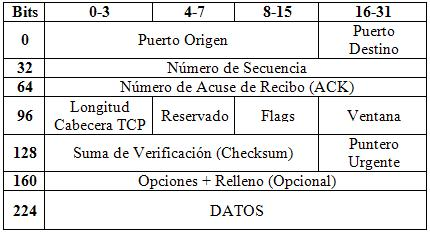
\includegraphics[height=4cm,width=0.6\textwidth]{parte_2/redes/cabecera-tcp} 
		\caption{Cabecera del protocolo TCP}
	\end{figure}

	En el encabezado TCP, se tiene puerto origen, puerto destino. Observando, el datagrama de la figura \ref{fig:datIP}, tenemos dos IPs: IP origen, e IP destino, y el protocolo TCP, tiene dos puertos(origen y destino), y el mismo protocolo. Este identificador de conexión se denomina 5-tupla,ya que cinco elementos son los que participan. 
	Por último, cabe destacar, que los puertos y los datos, los define el programador o software, en la capa de aplicación. El programador al usar el protocolo TCP, no debe realizar una verificación de los datos, ya que el protocolo mismo, se encarga de esto. 
	
	Estos elementos, se definen, ya que son necesarios para poder avanzar en los conceptos en el presente trabajo, ya que en un futuro, se deben configurar los software de los usuarios, y la programación del microcontrolador seleccionado en el capítulo anterior, basados en estos conceptos para poder realizar una integración exitosa, entre el microcontrolador y las computadoras del lugar. 
	
\section{Sniffer de red -WireShark} 

Un programa que pueda revisar los paquetes de una red que llegan a una computadora, y los pueda visualizar, se denomina sniffer. Un sniffer de red, no es mas que un software, en el cual se pueden visualizar los paquetes recibidos, en la computadora que esta instalado. El software elegido para realizar esta visualización de los paquetes se llama WireShark. Se ha elegido este software, dado que es software libre, y pueden filtrarse los paquetes por puertos, y por IP. Ademas tiene muchas otras opciones que no serán contadas, ya que no se utilizan en el desarrollo del dispositivo. En la primera pantalla, se debe seleccionar la placa de red de la PC (podría tener para de una), en la que se encuentra instalado, y luego puede realizar un análisis. A continuación se muestra una imagen de un análisis hecho sobre una PC.
%\setlength{\textheight}{290mm}
\begin{figure}[H]
	\centering 
	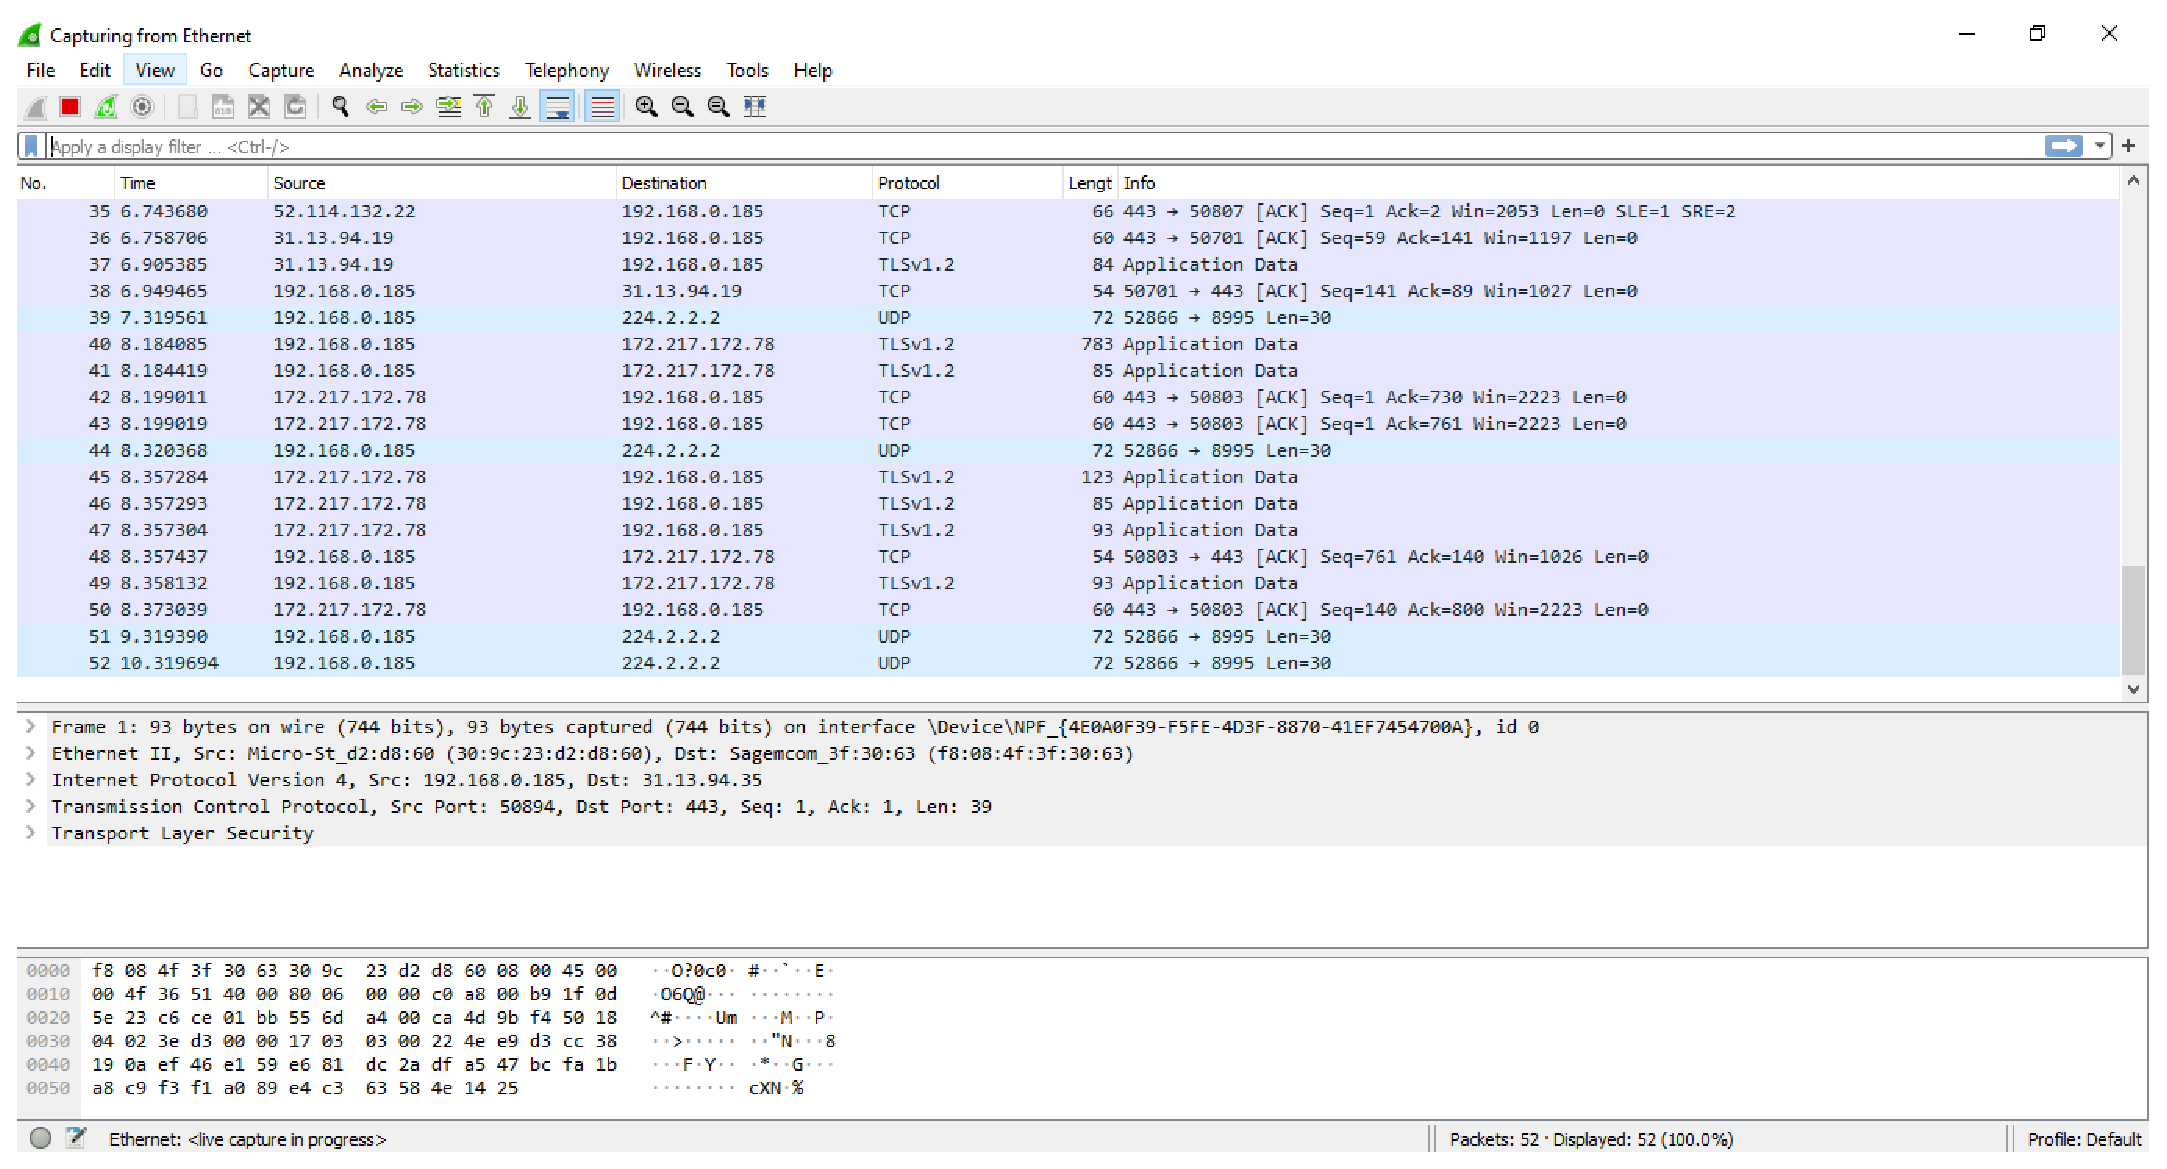
\includegraphics[height=7cm]{wireshark}
	\caption{análisis de los datos dentro de una red utilizando WireShark}
\end{figure}


Como se ve en la figura, se observa IP de origen, Ip de destino, y ambos puertos, y ademas el paquete TCP reensamblado, y el tipo de protocolo utilizado para la comunicación.  

Este software, se va a utilizar, para comprobar la conexión de los programas para que realicen seguimiento de satélites. Ademas, se puede comprobar los protocolos implementados por los programas. 

